% Created by tikzDevice version 0.12.3 on 2019-09-28 14:19:35
% !TEX encoding = UTF-8 Unicode
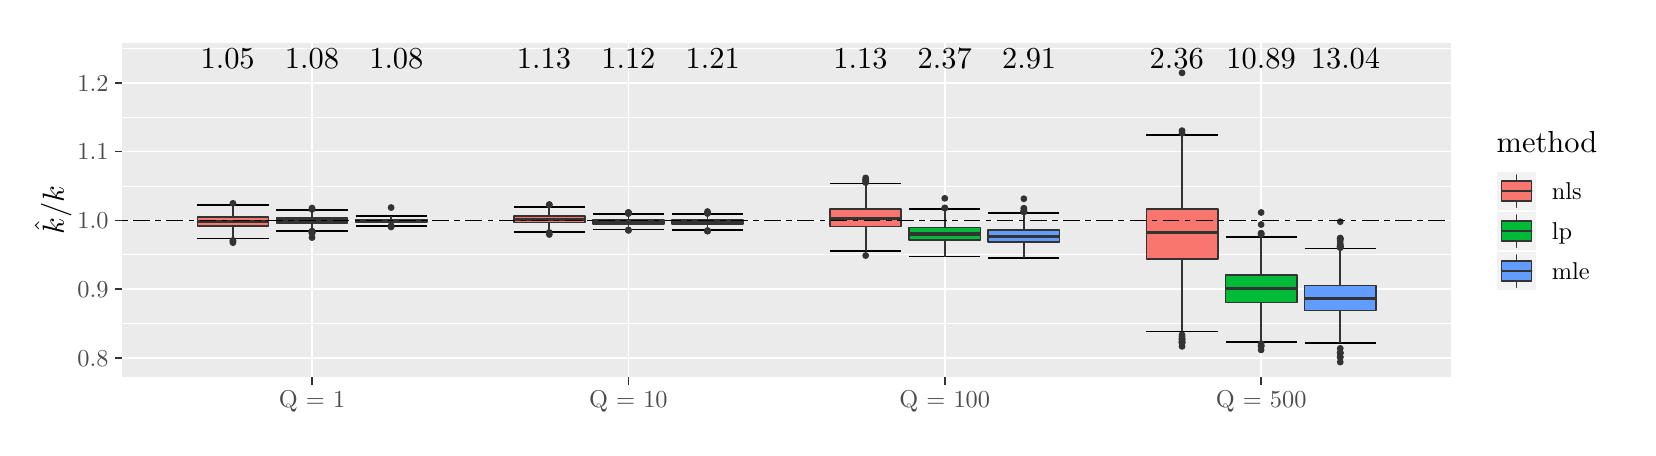
\begin{tikzpicture}[x=1pt,y=1pt]
\definecolor{fillColor}{RGB}{255,255,255}
\path[use as bounding box,fill=fillColor,fill opacity=0.00] (0,0) rectangle (578.16,144.54);
\begin{scope}
\path[clip] (  0.00,  0.00) rectangle (578.16,144.54);
\definecolor{drawColor}{RGB}{255,255,255}
\definecolor{fillColor}{RGB}{255,255,255}

\path[draw=drawColor,line width= 0.6pt,line join=round,line cap=round,fill=fillColor] (  0.00,  0.00) rectangle (578.16,144.54);
\end{scope}
\begin{scope}
\path[clip] ( 34.16, 18.22) rectangle (514.31,139.04);
\definecolor{fillColor}{gray}{0.92}

\path[fill=fillColor] ( 34.16, 18.22) rectangle (514.31,139.04);
\definecolor{drawColor}{RGB}{255,255,255}

\path[draw=drawColor,line width= 0.3pt,line join=round] ( 34.16, 37.56) --
	(514.31, 37.56);

\path[draw=drawColor,line width= 0.3pt,line join=round] ( 34.16, 62.44) --
	(514.31, 62.44);

\path[draw=drawColor,line width= 0.3pt,line join=round] ( 34.16, 87.33) --
	(514.31, 87.33);

\path[draw=drawColor,line width= 0.3pt,line join=round] ( 34.16,112.21) --
	(514.31,112.21);

\path[draw=drawColor,line width= 0.3pt,line join=round] ( 34.16,137.09) --
	(514.31,137.09);

\path[draw=drawColor,line width= 0.6pt,line join=round] ( 34.16, 25.12) --
	(514.31, 25.12);

\path[draw=drawColor,line width= 0.6pt,line join=round] ( 34.16, 50.00) --
	(514.31, 50.00);

\path[draw=drawColor,line width= 0.6pt,line join=round] ( 34.16, 74.88) --
	(514.31, 74.88);

\path[draw=drawColor,line width= 0.6pt,line join=round] ( 34.16, 99.77) --
	(514.31, 99.77);

\path[draw=drawColor,line width= 0.6pt,line join=round] ( 34.16,124.65) --
	(514.31,124.65);

\path[draw=drawColor,line width= 0.6pt,line join=round] (102.75, 18.22) --
	(102.75,139.04);

\path[draw=drawColor,line width= 0.6pt,line join=round] (217.07, 18.22) --
	(217.07,139.04);

\path[draw=drawColor,line width= 0.6pt,line join=round] (331.39, 18.22) --
	(331.39,139.04);

\path[draw=drawColor,line width= 0.6pt,line join=round] (445.71, 18.22) --
	(445.71,139.04);
\definecolor{drawColor}{RGB}{0,0,0}

\path[draw=drawColor,line width= 0.6pt,line join=round] ( 61.31, 80.51) --
	( 87.03, 80.51);

\path[draw=drawColor,line width= 0.6pt,line join=round] ( 74.17, 80.51) --
	( 74.17, 68.34);

\path[draw=drawColor,line width= 0.6pt,line join=round] ( 61.31, 68.34) --
	( 87.03, 68.34);

\path[draw=drawColor,line width= 0.6pt,line join=round] ( 89.89, 78.66) --
	(115.61, 78.66);

\path[draw=drawColor,line width= 0.6pt,line join=round] (102.75, 78.66) --
	(102.75, 71.03);

\path[draw=drawColor,line width= 0.6pt,line join=round] ( 89.89, 71.03) --
	(115.61, 71.03);

\path[draw=drawColor,line width= 0.6pt,line join=round] (118.47, 76.58) --
	(144.19, 76.58);

\path[draw=drawColor,line width= 0.6pt,line join=round] (131.33, 76.58) --
	(131.33, 72.98);

\path[draw=drawColor,line width= 0.6pt,line join=round] (118.47, 72.98) --
	(144.19, 72.98);

\path[draw=drawColor,line width= 0.6pt,line join=round] (175.63, 79.85) --
	(201.35, 79.85);

\path[draw=drawColor,line width= 0.6pt,line join=round] (188.49, 79.85) --
	(188.49, 70.61);

\path[draw=drawColor,line width= 0.6pt,line join=round] (175.63, 70.61) --
	(201.35, 70.61);

\path[draw=drawColor,line width= 0.6pt,line join=round] (204.21, 77.28) --
	(229.93, 77.28);

\path[draw=drawColor,line width= 0.6pt,line join=round] (217.07, 77.28) --
	(217.07, 71.55);

\path[draw=drawColor,line width= 0.6pt,line join=round] (204.21, 71.55) --
	(229.93, 71.55);

\path[draw=drawColor,line width= 0.6pt,line join=round] (232.79, 77.13) --
	(258.51, 77.13);

\path[draw=drawColor,line width= 0.6pt,line join=round] (245.65, 77.13) --
	(245.65, 71.49);

\path[draw=drawColor,line width= 0.6pt,line join=round] (232.79, 71.49) --
	(258.51, 71.49);

\path[draw=drawColor,line width= 0.6pt,line join=round] (289.95, 88.27) --
	(315.67, 88.27);

\path[draw=drawColor,line width= 0.6pt,line join=round] (302.81, 88.27) --
	(302.81, 63.81);

\path[draw=drawColor,line width= 0.6pt,line join=round] (289.95, 63.81) --
	(315.67, 63.81);

\path[draw=drawColor,line width= 0.6pt,line join=round] (318.53, 78.91) --
	(344.25, 78.91);

\path[draw=drawColor,line width= 0.6pt,line join=round] (331.39, 78.91) --
	(331.39, 61.81);

\path[draw=drawColor,line width= 0.6pt,line join=round] (318.53, 61.81) --
	(344.25, 61.81);

\path[draw=drawColor,line width= 0.6pt,line join=round] (347.11, 77.67) --
	(372.83, 77.67);

\path[draw=drawColor,line width= 0.6pt,line join=round] (359.97, 77.67) --
	(359.97, 61.26);

\path[draw=drawColor,line width= 0.6pt,line join=round] (347.11, 61.26) --
	(372.83, 61.26);

\path[draw=drawColor,line width= 0.6pt,line join=round] (404.27,105.71) --
	(430.00,105.71);

\path[draw=drawColor,line width= 0.6pt,line join=round] (417.13,105.71) --
	(417.13, 34.76);

\path[draw=drawColor,line width= 0.6pt,line join=round] (404.27, 34.76) --
	(430.00, 34.76);

\path[draw=drawColor,line width= 0.6pt,line join=round] (432.85, 68.98) --
	(458.58, 68.98);

\path[draw=drawColor,line width= 0.6pt,line join=round] (445.71, 68.98) --
	(445.71, 31.06);

\path[draw=drawColor,line width= 0.6pt,line join=round] (432.85, 31.06) --
	(458.58, 31.06);

\path[draw=drawColor,line width= 0.6pt,line join=round] (461.43, 64.79) --
	(487.16, 64.79);

\path[draw=drawColor,line width= 0.6pt,line join=round] (474.29, 64.79) --
	(474.29, 30.53);

\path[draw=drawColor,line width= 0.6pt,line join=round] (461.43, 30.53) --
	(487.16, 30.53);
\definecolor{drawColor}{gray}{0.20}
\definecolor{fillColor}{gray}{0.20}

\path[draw=drawColor,line width= 0.4pt,line join=round,line cap=round,fill=fillColor] ( 74.17, 66.85) circle (  1.02);

\path[draw=drawColor,line width= 0.4pt,line join=round,line cap=round,fill=fillColor] ( 74.17, 67.69) circle (  1.02);

\path[draw=drawColor,line width= 0.4pt,line join=round,line cap=round,fill=fillColor] ( 74.17, 67.37) circle (  1.02);

\path[draw=drawColor,line width= 0.4pt,line join=round,line cap=round,fill=fillColor] ( 74.17, 81.07) circle (  1.02);

\path[draw=drawColor,line width= 0.6pt,line join=round] ( 74.17, 76.04) -- ( 74.17, 80.51);

\path[draw=drawColor,line width= 0.6pt,line join=round] ( 74.17, 72.89) -- ( 74.17, 68.34);
\definecolor{fillColor}{RGB}{248,118,109}

\path[draw=drawColor,line width= 0.6pt,line join=round,line cap=round,fill=fillColor] ( 61.31, 76.04) --
	( 61.31, 72.89) --
	( 87.03, 72.89) --
	( 87.03, 76.04) --
	( 61.31, 76.04) --
	cycle;

\path[draw=drawColor,line width= 1.1pt,line join=round] ( 61.31, 74.52) -- ( 87.03, 74.52);
\definecolor{fillColor}{gray}{0.20}

\path[draw=drawColor,line width= 0.4pt,line join=round,line cap=round,fill=fillColor] (102.75, 70.39) circle (  1.02);

\path[draw=drawColor,line width= 0.4pt,line join=round,line cap=round,fill=fillColor] (102.75, 79.36) circle (  1.02);

\path[draw=drawColor,line width= 0.4pt,line join=round,line cap=round,fill=fillColor] (102.75, 68.69) circle (  1.02);

\path[draw=drawColor,line width= 0.4pt,line join=round,line cap=round,fill=fillColor] (102.75, 70.66) circle (  1.02);

\path[draw=drawColor,line width= 0.4pt,line join=round,line cap=round,fill=fillColor] (102.75, 70.98) circle (  1.02);

\path[draw=drawColor,line width= 0.4pt,line join=round,line cap=round,fill=fillColor] (102.75, 70.89) circle (  1.02);

\path[draw=drawColor,line width= 0.4pt,line join=round,line cap=round,fill=fillColor] (102.75, 70.82) circle (  1.02);

\path[draw=drawColor,line width= 0.4pt,line join=round,line cap=round,fill=fillColor] (102.75, 70.88) circle (  1.02);

\path[draw=drawColor,line width= 0.4pt,line join=round,line cap=round,fill=fillColor] (102.75, 70.78) circle (  1.02);

\path[draw=drawColor,line width= 0.4pt,line join=round,line cap=round,fill=fillColor] (102.75, 70.83) circle (  1.02);

\path[draw=drawColor,line width= 0.4pt,line join=round,line cap=round,fill=fillColor] (102.75, 70.24) circle (  1.02);

\path[draw=drawColor,line width= 0.4pt,line join=round,line cap=round,fill=fillColor] (102.75, 78.86) circle (  1.02);

\path[draw=drawColor,line width= 0.6pt,line join=round] (102.75, 75.80) -- (102.75, 78.66);

\path[draw=drawColor,line width= 0.6pt,line join=round] (102.75, 73.89) -- (102.75, 71.03);
\definecolor{fillColor}{RGB}{0,186,56}

\path[draw=drawColor,line width= 0.6pt,line join=round,line cap=round,fill=fillColor] ( 89.89, 75.80) --
	( 89.89, 73.89) --
	(115.61, 73.89) --
	(115.61, 75.80) --
	( 89.89, 75.80) --
	cycle;

\path[draw=drawColor,line width= 1.1pt,line join=round] ( 89.89, 74.82) -- (115.61, 74.82);
\definecolor{fillColor}{gray}{0.20}

\path[draw=drawColor,line width= 0.4pt,line join=round,line cap=round,fill=fillColor] (131.33, 72.65) circle (  1.02);

\path[draw=drawColor,line width= 0.4pt,line join=round,line cap=round,fill=fillColor] (131.33, 72.88) circle (  1.02);

\path[draw=drawColor,line width= 0.4pt,line join=round,line cap=round,fill=fillColor] (131.33, 72.54) circle (  1.02);

\path[draw=drawColor,line width= 0.4pt,line join=round,line cap=round,fill=fillColor] (131.33, 79.54) circle (  1.02);

\path[draw=drawColor,line width= 0.4pt,line join=round,line cap=round,fill=fillColor] (131.33, 72.96) circle (  1.02);

\path[draw=drawColor,line width= 0.6pt,line join=round] (131.33, 75.24) -- (131.33, 76.58);

\path[draw=drawColor,line width= 0.6pt,line join=round] (131.33, 74.33) -- (131.33, 72.98);
\definecolor{fillColor}{RGB}{97,156,255}

\path[draw=drawColor,line width= 0.6pt,line join=round,line cap=round,fill=fillColor] (118.47, 75.24) --
	(118.47, 74.33) --
	(144.19, 74.33) --
	(144.19, 75.24) --
	(118.47, 75.24) --
	cycle;

\path[draw=drawColor,line width= 1.1pt,line join=round] (118.47, 74.78) -- (144.19, 74.78);
\definecolor{fillColor}{gray}{0.20}

\path[draw=drawColor,line width= 0.4pt,line join=round,line cap=round,fill=fillColor] (188.49, 80.50) circle (  1.02);

\path[draw=drawColor,line width= 0.4pt,line join=round,line cap=round,fill=fillColor] (188.49, 70.54) circle (  1.02);

\path[draw=drawColor,line width= 0.4pt,line join=round,line cap=round,fill=fillColor] (188.49, 80.64) circle (  1.02);

\path[draw=drawColor,line width= 0.4pt,line join=round,line cap=round,fill=fillColor] (188.49, 69.81) circle (  1.02);

\path[draw=drawColor,line width= 0.6pt,line join=round] (188.49, 76.43) -- (188.49, 79.85);

\path[draw=drawColor,line width= 0.6pt,line join=round] (188.49, 74.08) -- (188.49, 70.61);
\definecolor{fillColor}{RGB}{248,118,109}

\path[draw=drawColor,line width= 0.6pt,line join=round,line cap=round,fill=fillColor] (175.63, 76.43) --
	(175.63, 74.08) --
	(201.35, 74.08) --
	(201.35, 76.43) --
	(175.63, 76.43) --
	cycle;

\path[draw=drawColor,line width= 1.1pt,line join=round] (175.63, 75.23) -- (201.35, 75.23);
\definecolor{fillColor}{gray}{0.20}

\path[draw=drawColor,line width= 0.4pt,line join=round,line cap=round,fill=fillColor] (217.07, 77.53) circle (  1.02);

\path[draw=drawColor,line width= 0.4pt,line join=round,line cap=round,fill=fillColor] (217.07, 71.46) circle (  1.02);

\path[draw=drawColor,line width= 0.4pt,line join=round,line cap=round,fill=fillColor] (217.07, 77.73) circle (  1.02);

\path[draw=drawColor,line width= 0.4pt,line join=round,line cap=round,fill=fillColor] (217.07, 77.68) circle (  1.02);

\path[draw=drawColor,line width= 0.4pt,line join=round,line cap=round,fill=fillColor] (217.07, 77.54) circle (  1.02);

\path[draw=drawColor,line width= 0.4pt,line join=round,line cap=round,fill=fillColor] (217.07, 77.38) circle (  1.02);

\path[draw=drawColor,line width= 0.4pt,line join=round,line cap=round,fill=fillColor] (217.07, 71.32) circle (  1.02);

\path[draw=drawColor,line width= 0.4pt,line join=round,line cap=round,fill=fillColor] (217.07, 77.45) circle (  1.02);

\path[draw=drawColor,line width= 0.4pt,line join=round,line cap=round,fill=fillColor] (217.07, 77.76) circle (  1.02);

\path[draw=drawColor,line width= 0.4pt,line join=round,line cap=round,fill=fillColor] (217.07, 71.33) circle (  1.02);

\path[draw=drawColor,line width= 0.6pt,line join=round] (217.07, 75.14) -- (217.07, 77.28);

\path[draw=drawColor,line width= 0.6pt,line join=round] (217.07, 73.68) -- (217.07, 71.55);
\definecolor{fillColor}{RGB}{0,186,56}

\path[draw=drawColor,line width= 0.6pt,line join=round,line cap=round,fill=fillColor] (204.21, 75.14) --
	(204.21, 73.68) --
	(229.93, 73.68) --
	(229.93, 75.14) --
	(204.21, 75.14) --
	cycle;

\path[draw=drawColor,line width= 1.1pt,line join=round] (204.21, 74.44) -- (229.93, 74.44);
\definecolor{fillColor}{gray}{0.20}

\path[draw=drawColor,line width= 0.4pt,line join=round,line cap=round,fill=fillColor] (245.65, 71.10) circle (  1.02);

\path[draw=drawColor,line width= 0.4pt,line join=round,line cap=round,fill=fillColor] (245.65, 77.47) circle (  1.02);

\path[draw=drawColor,line width= 0.4pt,line join=round,line cap=round,fill=fillColor] (245.65, 71.23) circle (  1.02);

\path[draw=drawColor,line width= 0.4pt,line join=round,line cap=round,fill=fillColor] (245.65, 77.58) circle (  1.02);

\path[draw=drawColor,line width= 0.4pt,line join=round,line cap=round,fill=fillColor] (245.65, 77.42) circle (  1.02);

\path[draw=drawColor,line width= 0.4pt,line join=round,line cap=round,fill=fillColor] (245.65, 71.05) circle (  1.02);

\path[draw=drawColor,line width= 0.4pt,line join=round,line cap=round,fill=fillColor] (245.65, 78.10) circle (  1.02);

\path[draw=drawColor,line width= 0.4pt,line join=round,line cap=round,fill=fillColor] (245.65, 71.09) circle (  1.02);

\path[draw=drawColor,line width= 0.6pt,line join=round] (245.65, 75.01) -- (245.65, 77.13);

\path[draw=drawColor,line width= 0.6pt,line join=round] (245.65, 73.52) -- (245.65, 71.49);
\definecolor{fillColor}{RGB}{97,156,255}

\path[draw=drawColor,line width= 0.6pt,line join=round,line cap=round,fill=fillColor] (232.79, 75.01) --
	(232.79, 73.52) --
	(258.51, 73.52) --
	(258.51, 75.01) --
	(232.79, 75.01) --
	cycle;

\path[draw=drawColor,line width= 1.1pt,line join=round] (232.79, 74.31) -- (258.51, 74.31);
\definecolor{fillColor}{gray}{0.20}

\path[draw=drawColor,line width= 0.4pt,line join=round,line cap=round,fill=fillColor] (302.81, 62.20) circle (  1.02);

\path[draw=drawColor,line width= 0.4pt,line join=round,line cap=round,fill=fillColor] (302.81, 89.63) circle (  1.02);

\path[draw=drawColor,line width= 0.4pt,line join=round,line cap=round,fill=fillColor] (302.81, 88.56) circle (  1.02);

\path[draw=drawColor,line width= 0.4pt,line join=round,line cap=round,fill=fillColor] (302.81, 88.99) circle (  1.02);

\path[draw=drawColor,line width= 0.4pt,line join=round,line cap=round,fill=fillColor] (302.81, 89.39) circle (  1.02);

\path[draw=drawColor,line width= 0.4pt,line join=round,line cap=round,fill=fillColor] (302.81, 90.25) circle (  1.02);

\path[draw=drawColor,line width= 0.6pt,line join=round] (302.81, 78.98) -- (302.81, 88.27);

\path[draw=drawColor,line width= 0.6pt,line join=round] (302.81, 72.73) -- (302.81, 63.81);
\definecolor{fillColor}{RGB}{248,118,109}

\path[draw=drawColor,line width= 0.6pt,line join=round,line cap=round,fill=fillColor] (289.95, 78.98) --
	(289.95, 72.73) --
	(315.67, 72.73) --
	(315.67, 78.98) --
	(289.95, 78.98) --
	cycle;

\path[draw=drawColor,line width= 1.1pt,line join=round] (289.95, 75.68) -- (315.67, 75.68);
\definecolor{fillColor}{gray}{0.20}

\path[draw=drawColor,line width= 0.4pt,line join=round,line cap=round,fill=fillColor] (331.39, 82.87) circle (  1.02);

\path[draw=drawColor,line width= 0.4pt,line join=round,line cap=round,fill=fillColor] (331.39, 79.35) circle (  1.02);

\path[draw=drawColor,line width= 0.4pt,line join=round,line cap=round,fill=fillColor] (331.39, 79.39) circle (  1.02);

\path[draw=drawColor,line width= 0.6pt,line join=round] (331.39, 72.34) -- (331.39, 78.91);

\path[draw=drawColor,line width= 0.6pt,line join=round] (331.39, 67.92) -- (331.39, 61.81);
\definecolor{fillColor}{RGB}{0,186,56}

\path[draw=drawColor,line width= 0.6pt,line join=round,line cap=round,fill=fillColor] (318.53, 72.34) --
	(318.53, 67.92) --
	(344.25, 67.92) --
	(344.25, 72.34) --
	(318.53, 72.34) --
	cycle;

\path[draw=drawColor,line width= 1.1pt,line join=round] (318.53, 69.98) -- (344.25, 69.98);
\definecolor{fillColor}{gray}{0.20}

\path[draw=drawColor,line width= 0.4pt,line join=round,line cap=round,fill=fillColor] (359.97, 77.98) circle (  1.02);

\path[draw=drawColor,line width= 0.4pt,line join=round,line cap=round,fill=fillColor] (359.97, 82.72) circle (  1.02);

\path[draw=drawColor,line width= 0.4pt,line join=round,line cap=round,fill=fillColor] (359.97, 79.20) circle (  1.02);

\path[draw=drawColor,line width= 0.4pt,line join=round,line cap=round,fill=fillColor] (359.97, 79.26) circle (  1.02);

\path[draw=drawColor,line width= 0.4pt,line join=round,line cap=round,fill=fillColor] (359.97, 78.13) circle (  1.02);

\path[draw=drawColor,line width= 0.4pt,line join=round,line cap=round,fill=fillColor] (359.97, 78.34) circle (  1.02);

\path[draw=drawColor,line width= 0.4pt,line join=round,line cap=round,fill=fillColor] (359.97, 78.10) circle (  1.02);

\path[draw=drawColor,line width= 0.4pt,line join=round,line cap=round,fill=fillColor] (359.97, 78.03) circle (  1.02);

\path[draw=drawColor,line width= 0.6pt,line join=round] (359.97, 71.40) -- (359.97, 77.67);

\path[draw=drawColor,line width= 0.6pt,line join=round] (359.97, 67.06) -- (359.97, 61.26);
\definecolor{fillColor}{RGB}{97,156,255}

\path[draw=drawColor,line width= 0.6pt,line join=round,line cap=round,fill=fillColor] (347.11, 71.40) --
	(347.11, 67.06) --
	(372.83, 67.06) --
	(372.83, 71.40) --
	(347.11, 71.40) --
	cycle;

\path[draw=drawColor,line width= 1.1pt,line join=round] (347.11, 69.07) -- (372.83, 69.07);
\definecolor{fillColor}{gray}{0.20}

\path[draw=drawColor,line width= 0.4pt,line join=round,line cap=round,fill=fillColor] (417.13, 31.19) circle (  1.02);

\path[draw=drawColor,line width= 0.4pt,line join=round,line cap=round,fill=fillColor] (417.13, 29.37) circle (  1.02);

\path[draw=drawColor,line width= 0.4pt,line join=round,line cap=round,fill=fillColor] (417.13, 30.66) circle (  1.02);

\path[draw=drawColor,line width= 0.4pt,line join=round,line cap=round,fill=fillColor] (417.13, 33.56) circle (  1.02);

\path[draw=drawColor,line width= 0.4pt,line join=round,line cap=round,fill=fillColor] (417.13, 30.60) circle (  1.02);

\path[draw=drawColor,line width= 0.4pt,line join=round,line cap=round,fill=fillColor] (417.13,106.38) circle (  1.02);

\path[draw=drawColor,line width= 0.4pt,line join=round,line cap=round,fill=fillColor] (417.13, 32.15) circle (  1.02);

\path[draw=drawColor,line width= 0.4pt,line join=round,line cap=round,fill=fillColor] (417.13, 32.09) circle (  1.02);

\path[draw=drawColor,line width= 0.4pt,line join=round,line cap=round,fill=fillColor] (417.13,128.22) circle (  1.02);

\path[draw=drawColor,line width= 0.4pt,line join=round,line cap=round,fill=fillColor] (417.13, 32.92) circle (  1.02);

\path[draw=drawColor,line width= 0.4pt,line join=round,line cap=round,fill=fillColor] (417.13, 31.06) circle (  1.02);

\path[draw=drawColor,line width= 0.4pt,line join=round,line cap=round,fill=fillColor] (417.13, 31.84) circle (  1.02);

\path[draw=drawColor,line width= 0.4pt,line join=round,line cap=round,fill=fillColor] (417.13,107.34) circle (  1.02);

\path[draw=drawColor,line width= 0.6pt,line join=round] (417.13, 79.02) -- (417.13,105.71);

\path[draw=drawColor,line width= 0.6pt,line join=round] (417.13, 60.95) -- (417.13, 34.76);
\definecolor{fillColor}{RGB}{248,118,109}

\path[draw=drawColor,line width= 0.6pt,line join=round,line cap=round,fill=fillColor] (404.27, 79.02) --
	(404.27, 60.95) --
	(430.00, 60.95) --
	(430.00, 79.02) --
	(404.27, 79.02) --
	cycle;

\path[draw=drawColor,line width= 1.1pt,line join=round] (404.27, 70.54) -- (430.00, 70.54);
\definecolor{fillColor}{gray}{0.20}

\path[draw=drawColor,line width= 0.4pt,line join=round,line cap=round,fill=fillColor] (445.71, 29.56) circle (  1.02);

\path[draw=drawColor,line width= 0.4pt,line join=round,line cap=round,fill=fillColor] (445.71, 28.10) circle (  1.02);

\path[draw=drawColor,line width= 0.4pt,line join=round,line cap=round,fill=fillColor] (445.71, 70.18) circle (  1.02);

\path[draw=drawColor,line width= 0.4pt,line join=round,line cap=round,fill=fillColor] (445.71, 29.43) circle (  1.02);

\path[draw=drawColor,line width= 0.4pt,line join=round,line cap=round,fill=fillColor] (445.71, 70.30) circle (  1.02);

\path[draw=drawColor,line width= 0.4pt,line join=round,line cap=round,fill=fillColor] (445.71, 77.75) circle (  1.02);

\path[draw=drawColor,line width= 0.4pt,line join=round,line cap=round,fill=fillColor] (445.71, 30.38) circle (  1.02);

\path[draw=drawColor,line width= 0.4pt,line join=round,line cap=round,fill=fillColor] (445.71, 69.90) circle (  1.02);

\path[draw=drawColor,line width= 0.4pt,line join=round,line cap=round,fill=fillColor] (445.71, 69.85) circle (  1.02);

\path[draw=drawColor,line width= 0.4pt,line join=round,line cap=round,fill=fillColor] (445.71, 73.41) circle (  1.02);

\path[draw=drawColor,line width= 0.4pt,line join=round,line cap=round,fill=fillColor] (445.71, 29.59) circle (  1.02);

\path[draw=drawColor,line width= 0.6pt,line join=round] (445.71, 55.06) -- (445.71, 68.98);

\path[draw=drawColor,line width= 0.6pt,line join=round] (445.71, 45.20) -- (445.71, 31.06);
\definecolor{fillColor}{RGB}{0,186,56}

\path[draw=drawColor,line width= 0.6pt,line join=round,line cap=round,fill=fillColor] (432.85, 55.06) --
	(432.85, 45.20) --
	(458.58, 45.20) --
	(458.58, 55.06) --
	(432.85, 55.06) --
	cycle;

\path[draw=drawColor,line width= 1.1pt,line join=round] (432.85, 50.22) -- (458.58, 50.22);
\definecolor{fillColor}{gray}{0.20}

\path[draw=drawColor,line width= 0.4pt,line join=round,line cap=round,fill=fillColor] (474.29, 67.49) circle (  1.02);

\path[draw=drawColor,line width= 0.4pt,line join=round,line cap=round,fill=fillColor] (474.29, 68.32) circle (  1.02);

\path[draw=drawColor,line width= 0.4pt,line join=round,line cap=round,fill=fillColor] (474.29, 28.65) circle (  1.02);

\path[draw=drawColor,line width= 0.4pt,line join=round,line cap=round,fill=fillColor] (474.29, 68.52) circle (  1.02);

\path[draw=drawColor,line width= 0.4pt,line join=round,line cap=round,fill=fillColor] (474.29, 74.43) circle (  1.02);

\path[draw=drawColor,line width= 0.4pt,line join=round,line cap=round,fill=fillColor] (474.29, 65.45) circle (  1.02);

\path[draw=drawColor,line width= 0.4pt,line join=round,line cap=round,fill=fillColor] (474.29, 25.39) circle (  1.02);

\path[draw=drawColor,line width= 0.4pt,line join=round,line cap=round,fill=fillColor] (474.29, 25.60) circle (  1.02);

\path[draw=drawColor,line width= 0.4pt,line join=round,line cap=round,fill=fillColor] (474.29, 68.29) circle (  1.02);

\path[draw=drawColor,line width= 0.4pt,line join=round,line cap=round,fill=fillColor] (474.29, 66.47) circle (  1.02);

\path[draw=drawColor,line width= 0.4pt,line join=round,line cap=round,fill=fillColor] (474.29, 65.42) circle (  1.02);

\path[draw=drawColor,line width= 0.4pt,line join=round,line cap=round,fill=fillColor] (474.29, 65.19) circle (  1.02);

\path[draw=drawColor,line width= 0.4pt,line join=round,line cap=round,fill=fillColor] (474.29, 68.22) circle (  1.02);

\path[draw=drawColor,line width= 0.4pt,line join=round,line cap=round,fill=fillColor] (474.29, 65.49) circle (  1.02);

\path[draw=drawColor,line width= 0.4pt,line join=round,line cap=round,fill=fillColor] (474.29, 23.71) circle (  1.02);

\path[draw=drawColor,line width= 0.4pt,line join=round,line cap=round,fill=fillColor] (474.29, 27.12) circle (  1.02);

\path[draw=drawColor,line width= 0.4pt,line join=round,line cap=round,fill=fillColor] (474.29, 65.04) circle (  1.02);

\path[draw=drawColor,line width= 0.4pt,line join=round,line cap=round,fill=fillColor] (474.29, 26.97) circle (  1.02);

\path[draw=drawColor,line width= 0.4pt,line join=round,line cap=round,fill=fillColor] (474.29, 65.96) circle (  1.02);

\path[draw=drawColor,line width= 0.4pt,line join=round,line cap=round,fill=fillColor] (474.29, 27.07) circle (  1.02);

\path[draw=drawColor,line width= 0.6pt,line join=round] (474.29, 51.42) -- (474.29, 64.79);

\path[draw=drawColor,line width= 0.6pt,line join=round] (474.29, 42.40) -- (474.29, 30.53);
\definecolor{fillColor}{RGB}{97,156,255}

\path[draw=drawColor,line width= 0.6pt,line join=round,line cap=round,fill=fillColor] (461.43, 51.42) --
	(461.43, 42.40) --
	(487.16, 42.40) --
	(487.16, 51.42) --
	(461.43, 51.42) --
	cycle;

\path[draw=drawColor,line width= 1.1pt,line join=round] (461.43, 46.76) -- (487.16, 46.76);
\definecolor{drawColor}{RGB}{0,0,0}

\path[draw=drawColor,line width= 0.6pt,dash pattern=on 2pt off 2pt on 6pt off 2pt ,line join=round] ( 34.16, 74.88) -- (514.31, 74.88);

\node[text=drawColor,anchor=base,inner sep=0pt, outer sep=0pt, scale=  1.10] at (133.23,129.75) {1.08};

\node[text=drawColor,anchor=base,inner sep=0pt, outer sep=0pt, scale=  1.10] at (102.75,129.75) {1.08};

\node[text=drawColor,anchor=base,inner sep=0pt, outer sep=0pt, scale=  1.10] at ( 72.26,129.75) {1.05};

\node[text=drawColor,anchor=base,inner sep=0pt, outer sep=0pt, scale=  1.10] at (247.56,129.75) {1.21};

\node[text=drawColor,anchor=base,inner sep=0pt, outer sep=0pt, scale=  1.10] at (217.07,129.75) {1.12};

\node[text=drawColor,anchor=base,inner sep=0pt, outer sep=0pt, scale=  1.10] at (186.59,129.75) {1.13};

\node[text=drawColor,anchor=base,inner sep=0pt, outer sep=0pt, scale=  1.10] at (361.88,129.75) {2.91};

\node[text=drawColor,anchor=base,inner sep=0pt, outer sep=0pt, scale=  1.10] at (331.39,129.75) {2.37};

\node[text=drawColor,anchor=base,inner sep=0pt, outer sep=0pt, scale=  1.10] at (300.91,129.75) {1.13};

\node[text=drawColor,anchor=base,inner sep=0pt, outer sep=0pt, scale=  1.10] at (476.20,129.75) {13.04};

\node[text=drawColor,anchor=base,inner sep=0pt, outer sep=0pt, scale=  1.10] at (445.71,129.75) {10.89};

\node[text=drawColor,anchor=base,inner sep=0pt, outer sep=0pt, scale=  1.10] at (415.23,129.75) {2.36};
\end{scope}
\begin{scope}
\path[clip] (  0.00,  0.00) rectangle (578.16,144.54);
\definecolor{drawColor}{gray}{0.30}

\node[text=drawColor,anchor=base east,inner sep=0pt, outer sep=0pt, scale=  0.88] at ( 29.21, 22.09) {0.8};

\node[text=drawColor,anchor=base east,inner sep=0pt, outer sep=0pt, scale=  0.88] at ( 29.21, 46.97) {0.9};

\node[text=drawColor,anchor=base east,inner sep=0pt, outer sep=0pt, scale=  0.88] at ( 29.21, 71.85) {1.0};

\node[text=drawColor,anchor=base east,inner sep=0pt, outer sep=0pt, scale=  0.88] at ( 29.21, 96.74) {1.1};

\node[text=drawColor,anchor=base east,inner sep=0pt, outer sep=0pt, scale=  0.88] at ( 29.21,121.62) {1.2};
\end{scope}
\begin{scope}
\path[clip] (  0.00,  0.00) rectangle (578.16,144.54);
\definecolor{drawColor}{gray}{0.20}

\path[draw=drawColor,line width= 0.6pt,line join=round] ( 31.41, 25.12) --
	( 34.16, 25.12);

\path[draw=drawColor,line width= 0.6pt,line join=round] ( 31.41, 50.00) --
	( 34.16, 50.00);

\path[draw=drawColor,line width= 0.6pt,line join=round] ( 31.41, 74.88) --
	( 34.16, 74.88);

\path[draw=drawColor,line width= 0.6pt,line join=round] ( 31.41, 99.77) --
	( 34.16, 99.77);

\path[draw=drawColor,line width= 0.6pt,line join=round] ( 31.41,124.65) --
	( 34.16,124.65);
\end{scope}
\begin{scope}
\path[clip] (  0.00,  0.00) rectangle (578.16,144.54);
\definecolor{drawColor}{gray}{0.20}

\path[draw=drawColor,line width= 0.6pt,line join=round] (102.75, 15.47) --
	(102.75, 18.22);

\path[draw=drawColor,line width= 0.6pt,line join=round] (217.07, 15.47) --
	(217.07, 18.22);

\path[draw=drawColor,line width= 0.6pt,line join=round] (331.39, 15.47) --
	(331.39, 18.22);

\path[draw=drawColor,line width= 0.6pt,line join=round] (445.71, 15.47) --
	(445.71, 18.22);
\end{scope}
\begin{scope}
\path[clip] (  0.00,  0.00) rectangle (578.16,144.54);
\definecolor{drawColor}{gray}{0.30}

\node[text=drawColor,anchor=base,inner sep=0pt, outer sep=0pt, scale=  0.88] at (102.75,  7.21) {Q = 1};

\node[text=drawColor,anchor=base,inner sep=0pt, outer sep=0pt, scale=  0.88] at (217.07,  7.21) {Q = 10};

\node[text=drawColor,anchor=base,inner sep=0pt, outer sep=0pt, scale=  0.88] at (331.39,  7.21) {Q = 100};

\node[text=drawColor,anchor=base,inner sep=0pt, outer sep=0pt, scale=  0.88] at (445.71,  7.21) {Q = 500};
\end{scope}
\begin{scope}
\path[clip] (  0.00,  0.00) rectangle (578.16,144.54);
\definecolor{drawColor}{RGB}{0,0,0}

\node[text=drawColor,rotate= 90.00,anchor=base,inner sep=0pt, outer sep=0pt, scale=  1.10] at ( 13.08, 78.63) {$\hat{k}/k$};
\end{scope}
\begin{scope}
\path[clip] (  0.00,  0.00) rectangle (578.16,144.54);
\definecolor{fillColor}{RGB}{255,255,255}

\path[fill=fillColor] (525.31, 43.84) rectangle (572.66,113.42);
\end{scope}
\begin{scope}
\path[clip] (  0.00,  0.00) rectangle (578.16,144.54);
\definecolor{drawColor}{RGB}{0,0,0}

\node[text=drawColor,anchor=base west,inner sep=0pt, outer sep=0pt, scale=  1.10] at (530.81, 99.27) {method};
\end{scope}
\begin{scope}
\path[clip] (  0.00,  0.00) rectangle (578.16,144.54);
\definecolor{drawColor}{RGB}{255,255,255}
\definecolor{fillColor}{gray}{0.95}

\path[draw=drawColor,line width= 0.6pt,line join=round,line cap=round,fill=fillColor] (530.81, 78.25) rectangle (545.26, 92.70);
\end{scope}
\begin{scope}
\path[clip] (  0.00,  0.00) rectangle (578.16,144.54);
\definecolor{drawColor}{gray}{0.20}

\path[draw=drawColor,line width= 0.6pt,line join=round,line cap=round] (538.03, 79.70) --
	(538.03, 81.86);

\path[draw=drawColor,line width= 0.6pt,line join=round,line cap=round] (538.03, 89.09) --
	(538.03, 91.26);
\definecolor{fillColor}{RGB}{248,118,109}

\path[draw=drawColor,line width= 0.6pt,line join=round,line cap=round,fill=fillColor] (532.61, 81.86) rectangle (543.45, 89.09);

\path[draw=drawColor,line width= 0.6pt,line join=round,line cap=round] (532.61, 85.48) --
	(543.45, 85.48);
\end{scope}
\begin{scope}
\path[clip] (  0.00,  0.00) rectangle (578.16,144.54);
\definecolor{drawColor}{RGB}{255,255,255}
\definecolor{fillColor}{gray}{0.95}

\path[draw=drawColor,line width= 0.6pt,line join=round,line cap=round,fill=fillColor] (530.81, 63.80) rectangle (545.26, 78.25);
\end{scope}
\begin{scope}
\path[clip] (  0.00,  0.00) rectangle (578.16,144.54);
\definecolor{drawColor}{gray}{0.20}

\path[draw=drawColor,line width= 0.6pt,line join=round,line cap=round] (538.03, 65.24) --
	(538.03, 67.41);

\path[draw=drawColor,line width= 0.6pt,line join=round,line cap=round] (538.03, 74.64) --
	(538.03, 76.81);
\definecolor{fillColor}{RGB}{0,186,56}

\path[draw=drawColor,line width= 0.6pt,line join=round,line cap=round,fill=fillColor] (532.61, 67.41) rectangle (543.45, 74.64);

\path[draw=drawColor,line width= 0.6pt,line join=round,line cap=round] (532.61, 71.02) --
	(543.45, 71.02);
\end{scope}
\begin{scope}
\path[clip] (  0.00,  0.00) rectangle (578.16,144.54);
\definecolor{drawColor}{RGB}{255,255,255}
\definecolor{fillColor}{gray}{0.95}

\path[draw=drawColor,line width= 0.6pt,line join=round,line cap=round,fill=fillColor] (530.81, 49.34) rectangle (545.26, 63.80);
\end{scope}
\begin{scope}
\path[clip] (  0.00,  0.00) rectangle (578.16,144.54);
\definecolor{drawColor}{gray}{0.20}

\path[draw=drawColor,line width= 0.6pt,line join=round,line cap=round] (538.03, 50.79) --
	(538.03, 52.96);

\path[draw=drawColor,line width= 0.6pt,line join=round,line cap=round] (538.03, 60.18) --
	(538.03, 62.35);
\definecolor{fillColor}{RGB}{97,156,255}

\path[draw=drawColor,line width= 0.6pt,line join=round,line cap=round,fill=fillColor] (532.61, 52.96) rectangle (543.45, 60.18);

\path[draw=drawColor,line width= 0.6pt,line join=round,line cap=round] (532.61, 56.57) --
	(543.45, 56.57);
\end{scope}
\begin{scope}
\path[clip] (  0.00,  0.00) rectangle (578.16,144.54);
\definecolor{drawColor}{RGB}{0,0,0}

\node[text=drawColor,anchor=base west,inner sep=0pt, outer sep=0pt, scale=  0.88] at (550.76, 82.45) {nls};
\end{scope}
\begin{scope}
\path[clip] (  0.00,  0.00) rectangle (578.16,144.54);
\definecolor{drawColor}{RGB}{0,0,0}

\node[text=drawColor,anchor=base west,inner sep=0pt, outer sep=0pt, scale=  0.88] at (550.76, 67.99) {lp};
\end{scope}
\begin{scope}
\path[clip] (  0.00,  0.00) rectangle (578.16,144.54);
\definecolor{drawColor}{RGB}{0,0,0}

\node[text=drawColor,anchor=base west,inner sep=0pt, outer sep=0pt, scale=  0.88] at (550.76, 53.54) {mle};
\end{scope}
\end{tikzpicture}
